% Chapter Template

\chapter{Data Pre-processing} % Main chapter title

\label{Chapter2} % Change X to a consecutive number; for referencing this chapter elsewhere, use \ref{ChapterX}

\section{Missing Values}

At the very beginning, the figure below shows the head of the original data set.

\begin{figure}[htbp!]
\centering
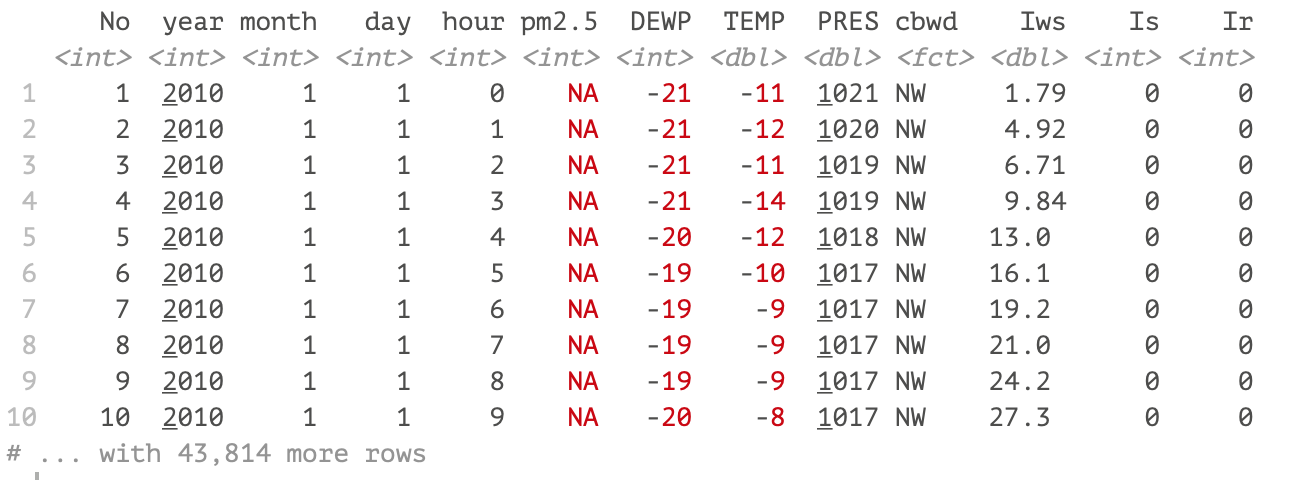
\includegraphics[width=1.0\textwidth]{Figures/origindata.png}
\caption[Figures/origindata.png]{Origin Data Set}
\label{fig:Origin data Set}
\end{figure}

\begin{figure}[htbp!]
\centering
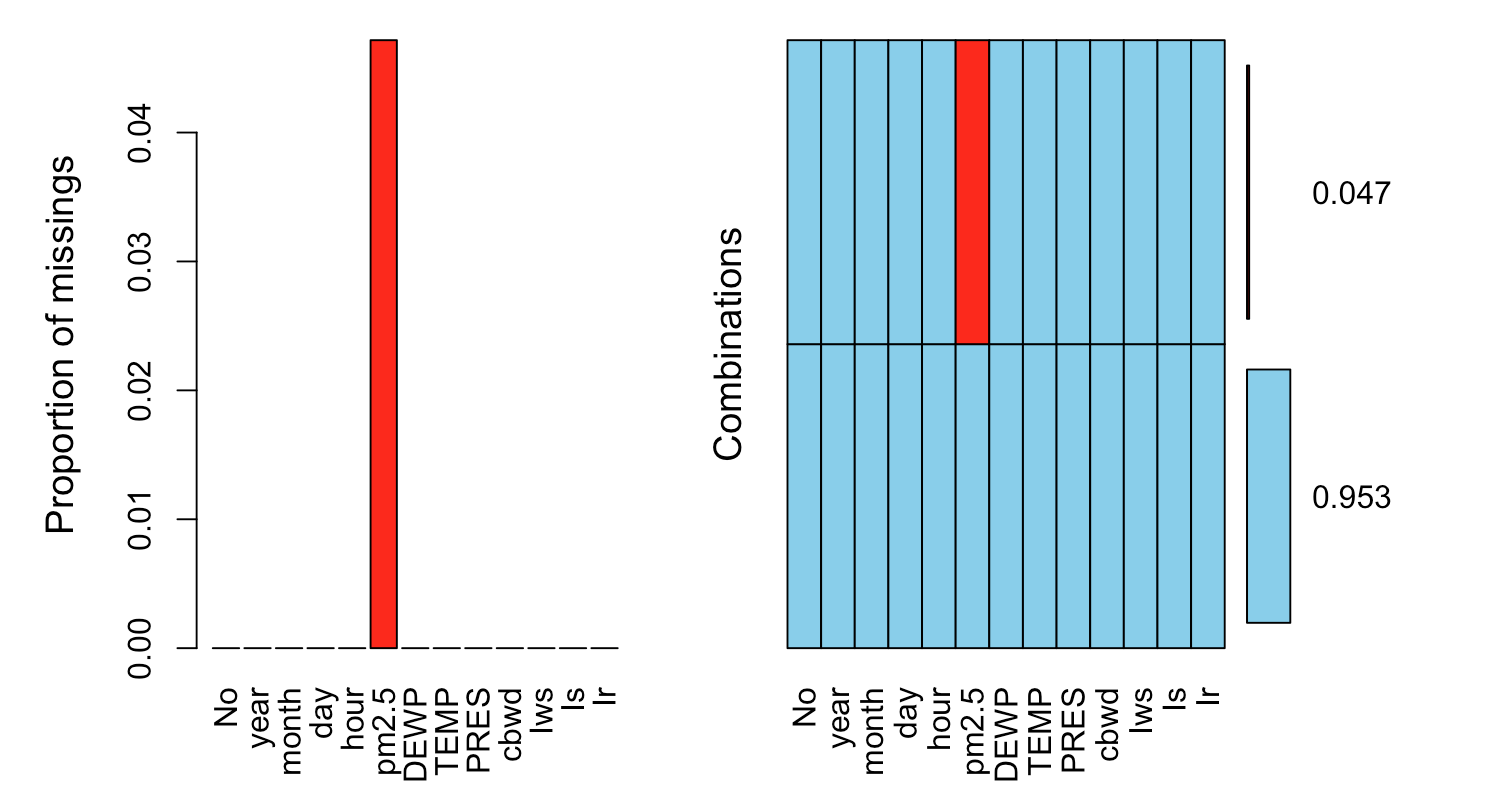
\includegraphics[width=1.0\textwidth]{Figures/missing.png}
\caption[Figures/missing.png]{Visualization of Missing Value}
\label{fig:missing}
\end{figure}

The data set we chosen is from the UCI Machine Learning Repository datasets, it has collected Beijing PM2.5 data from 2010 to 2014. In this data sets, its collection is based on hours, and from the original data set we can see that there are lots of missing value (approximately $4.7\%$ data of PM2.5 are missing). We need to delete the missing data. In order to reduce the impact of deleting missing values on data, we select the data of the fourth year and fifth year, namely 2013 and 2014 respectively.


\section{Time Data Processing}
As we have mentioned before, the PM2.5 maybe have a high co-linearity with time (a few hours a day, a few days a month, a few months a year), and in the time-series data, there usually auto-correlation between the  in order to ignore this time series problem, we decided to reduce this correlation through some data processing procedures.

After setting up the full model, we discover that the R square is insignificant, then we separate the data into two classes: Summer and Autumn, Spring and Winter. We do the model estimation. Then, we classified them again and now the data are in four classes. In order to select the most appropriate categorical variable, we believe that the PM2.5 level is related to the weather. For weather data, it is usually seasonal. For example, we expect winter air pollution to become more severe as coal consumption increases. Therefore, we decided to change only the classification predictor for the seasons to categorical variables.

At the same time, the wind direction and wind force will also affect the concentration of PM2.5 every day. Since the original data set has no wind data, only the hourly wind direction, and the current data set needs the average wind direction of each day, and the average wind direction calculation. It is divided into two methods, the averaging method and the vector summation method \citep{yueh1997modeling}. In order to eliminate the "wind strength" required in the "vector summation method", we choose to use the averaging method for calculation.

In addition, through the lubridate package in the R language, we convert the character variable "time" into a numeric variable: timestamp.

In the end, the new data set contains eight independent variables and one dependent variables:

\begin{figure}[h!]
\centering
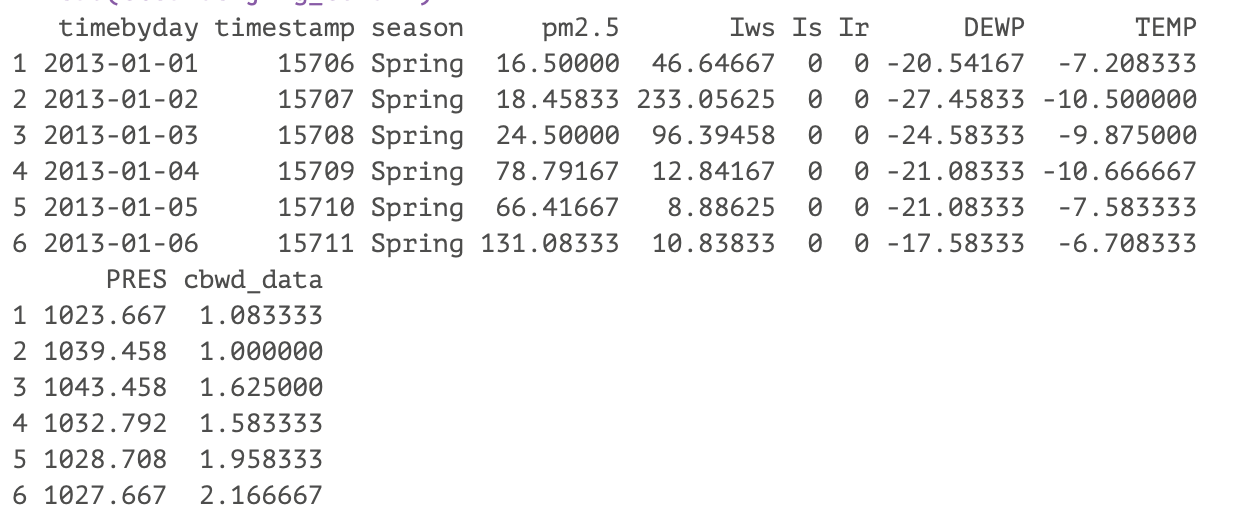
\includegraphics[width=1.0\textwidth]{Figures/newdata.png}
\caption[Figures/newdata.png]{new data set}
\label{fig:new data set}
\end{figure}
